\chapter{Marco metodológico}
\label{capitulo2}
\lhead{Capítulo 2. \emph{Marco metodológico}}

En este capítulo se detalla la representación utilizada para los cromosomas, la función objetivo, las adaptaciones particulares que se hizo a cada algoritmo evolutivo usado en el experimento, el proceso de validación cruzada, la técnica de estratificación y se presentan los conjuntos de datos usados para el experimento.

\section{Representación del cromosoma}

La representación usada para modelar el problema de selección de prototipos es el de un mapa de bits de tamaño $n$ igual al número de instancias pertenecientes al conjunto original, donde cada bit representa una instancia $t_i$; si el valor del bit i es 1, entonces la instancia $t_i \in S$, donde S es el conjunto reducido; si el bit i es 0, $t_i \notin S$. En este sentido, el conjunto S representado por el mapa de bits M se define como en la ecuación (2.1). Un ejemplo puede verse en la figura \ref{representacion}. Cabe destacar que en los algoritmos evolutivos, los mapas de bits se conocen como cromosomas y cada bit como gen.

\begin{equation}
S = \left\{ i \mid i = 1 \dots n \land m_i = 1 \land m_i \in M \right\}
\end{equation} 

\begin{figure}[]
\centering
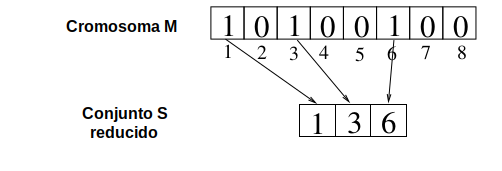
\includegraphics[height=3cm,width=10cm]{representacion.png}
\caption[Representación de un cromosoma y su respectivo conjunto reducido]{Representación de un cromosoma y su respectivo conjunto reducido}
\label{representacion}
\end{figure}

\section{Función objetivo}

Se necesita una función con la cual se pueda evaluar cuán buena es una solución, además la función debe permitir establecer una relación de orden entre las soluciones con el fin de decidir cuál solución es mejor. Como se explicó en la sección 1.3.2.1, los algoritmos evolutivos buscan aproximarse al óptimo global, que en este caso es el conjunto reducido S con menor cardinalidad y mayor precisión en la clasificación de instancias nuevas. Es por eso que se adopta una función objetivo derivada del trabajo de \emph{Cano, J.} en \cite{de2004reduccion}, la cual se presenta a continuación:

\begin{equation}
\mathcal{F}(S) = \alpha * error(S) + (1 - \alpha) * reduction(S)
\end{equation} 

Donde $\mathcal{F}: S \rightarrow \mathbb{R}$ es la función objetivo, S es el conjunto reducido, $\alpha$ es un parámetro que controla cuánta importancia se le da al error asociado a S con respecto a la tasa de reducción del segundo término de la ecuación (2.2). \emph{Error(S)} es el número de instancias clasificadas erróneamente cuando se usa el conjunto S como conjunto de entrenamiento de un clasificador 1-NN y \emph{reduction(S)} es el número de instancias en S dividido entre el número de instancias del conjunto original. El $\alpha$ usado es 0.5 como lo establecen en \cite{de2004reduccion} para darle la misma importancia a la reducción de datos como a mantener bajo los porcentajes de error en la clasificación.

Dado esta función objetivo, la meta de todas las metaheurísticas implementadas se vuelve minimizar $\mathcal{F}(S)$, lo que quiere decir que se busca tanto reducir la cardinalidad de $S$, como reducir error(S). Un conjunto $S_i$ es mejor que un conjunto $S_j$ si $\mathcal{F}(S_i) < \mathcal{F}(S_j)$.  

\section{Adaptaciones de los algoritmos evolutivos}

Para aplicar los distintos algoritmos evolutivos implementados para este trabajo, es necesario determinar los operadores de cruce, mutación, el método de selección de los cromosomas que van a cruzarse, el criterio de selección de los cromosomas sobrevivientes y en caso del algoritmo memético el proceso de optimización interno (también conocido como meme) utilizado.

Para el caso del algoritmo genético estacionario y el algoritmo memético, se eligió como método de selección de cromosomas a cruzarse un \emph{Proceso de Torneo} \cite{talbi2009metaheuristics}, el cual consiste en seleccionar $k$ cromosomas de manera aleatoria y elegir el mejor de los $k$. CHC por su parte elige dos cromosomas aleatorios y utiliza su mecanismo de prevención de incesto para elegir a los padres. El algoritmo genético generacional simplemente elige dos elementos aleatorios para realizar el cruce.

El operador de cruce utilizado en GGA, SSGA y MA es el cruce de un punto \cite{talbi2009metaheuristics}, el cual consiste en definir un punto $\mu$ en el cual se va dividir los dos cromosomas seleccionados como padres y luego se forman dos hijos a partir de la mezcla de las partes de los padres. CHC en cambio usa el operador HUX. En la figura \ref{cruce} se muestra un ejemplo del cruce de un punto. 

\begin{figure}[h!]
\centering
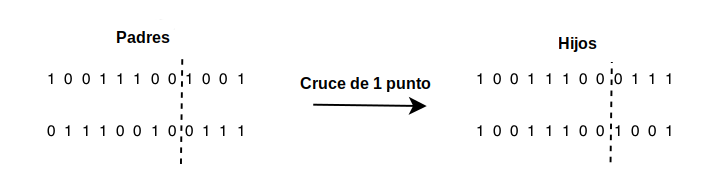
\includegraphics[width=\textwidth]{cruce.png}
\caption[Cruce de un punto]{Cruce de un punto}
\label{cruce}
\end{figure}

El operador de mutación para GGA, SSGA y MA consiste en cambiar 5\% de los genes del cromosoma de manera aleatoria. Se elige 5\%  basado en \cite{flores2014metaheuristics} para que la mutación represente una variación en S, ya que si sólo se cambia un gen, el conjunto mutado sería para los efectos de la optimización casi idéntico al original. Sin embargo, la probabilidad de que un cromosoma mute es baja, basado principalmente en los resultados de \emph{Cano, J.} en \cite{de2004reduccion} donde obtienen mejores resultados experimentales con bajas probabilidades de mutación (menor al 1\% por cromosoma), justificándose en que con mayores valores, la búsqueda podría degenerar en una búsqueda aleatoria. CHC por su parte no tiene mutación.

El criterio de reemplazo para GGA es generar una población nueva de hijos $P_i$ que va a suplantar la generación anterior $P_{i-1}$ excepto el mejor cromosoma en $P_{i-1}$. Por su parte, el criterio de reemplazo de SSGA es que dado dos padres y los dos hijos producidos por el operador de cruce, se eligen los 2 mejores cromosomas entre los padres e hijos para permanecer dentro de la población. MA, en cambio usa un criterio de reemplazo en el cual los 2 hijos suplantan a los 2 peores elementos de la población y CHC se queda con los \texttt{n} mejores cromosomas entre $P_i$ y $P_{i-1}$. Tanto MA como CHC son totalmente elitistas.

El algoritmo memético es el que más adaptaciones tiene para adecuarse a PS, se usa una adaptación realizada por \emph{Cano, J. et al.} en \cite{garcia2008memetic}. Se basa en el algoritmo memético estacionario presentado en la sección 1.3.2.1.3, con la peculiariadad de que para decidir si los hijos producidos en una iteración van a ser optimizados, se usa el parámetro $P_{LS}$ que viene dado por la siguiente ecuación:

\begin{equation}
P_{LS}=
\begin{cases}
1 & \text{si } \mathcal{F}(S_{nuevo}) < \mathcal{F}(S_{peor})\\
0.0625 & \text{en caso contrario}\\
\end{cases}
\end{equation}

Donde $\mathcal{F}$ es la función objetivo, $S_{nuevo}$ es el conjunto de uno de los cromosomas hijos y $S_{peor}$ es el conjunto del peor cromosoma de la población. Es así como $P_{LS}$ representa la probabilidad con la cual se va a decidir si se optimiza el cromosoma hijo; $P_{LS}$ debe ser calculado para cada hijo creado en el cruce. La idea es que si el hijo es mejor que el peor cromosoma de la población, entonces vale la pena optimizarlo; en cambio, si es peor, se le da una probabilidad de optimización de 6,25\%.

El meme usado en MA es el que se presenta en el algoritmo \ref{meme}. El procedimiento consiste en reducir progresivamente las instancias que se encuentran en el conjunto S, representado por el cromosoma M, sin que se pierda la precisión asociada a S. Para esto, se usa una lista U del primer vecino más cercano de cada gen en M, una lista R que contiene los genes que ya han sido colocados en 0 y que no generan una ganancia mayor al umbral de aceptación \texttt{t}, clase(i) es la clase asociada a la instancia representada por el gen i del cromosoma M, \texttt{ganancia} representa cuánto mejora (en caso de que sea positiva) o cuánto empeora (en caso de ser negativa) la solución dada por el cromosoma M luego de cambiar un gen, $fitness_M$ es el valor de evaluar la función objetivo con el cromosoma M y $fitness_{ganancia}$ se define como en la ecuación (2.4), donde L es el largo del cromosoma:

\begin{equation}
fitness_{ganancia} = \frac{\frac{ganancia}{L}*100 + \frac{100}{L}}{2}
\end{equation}  

El meme intenta remover una instancia de S en cada iteración para evaluar si la precisión mejora, se mantiene igual o empeora. Si la ganancia mejora, es decir que sea positiva, y está por encima del umbral de aceptación entonces se preservan los cambios; en cambio, si la ganancia está por debajo del umbral, entonces se vuelve a incluir la instancia eliminada y se etiqueta su respectivo gen como revisado.
 
\begin{algorithm}
\caption{Meme}
\label{meme}
\begin{algorithmic}[1]

\Require{\texttt{M} cromosoma a optimizar, \texttt{t} umbral de aceptación}
\Ensure{\texttt{M} cromosoma optimizado}

\State Sea $\texttt{M} = \left\{ m_1,m_2,\dots,m_n \right\}$ el cromosoma a optimizar 
\State $R \gets \emptyset$
\State $ U = \left\{ u_1,u_2,\dots,u_n \right\}$ la lista de vecinos asociados, donde $u_i$ es el vecino más cercano del gen i. 
\While{$(\exists m_i \in \texttt{M} \mid m_i = 1 \land i \notin R)$}
	\State elegir j aleatoriamente de \texttt{M} tal que $m_j=1 \land j \notin R$
	\State $ganancia \gets 0$
	\State $m_j \gets 0$
	\State Copiar U a U'
	\ForAll{$u_i \in U \mid u_i = j$}
		\State $u_i \gets$ nuevo vecino más cercano con el nuevo \texttt{M}
		\If{$clase(i) = clase(u'_i) \land clase(i) \neq clase(u_i)$}
			\State $ganancia \gets ganancia - 1$
		\ElsIf{$clase(i) \neq clase(u'_i) \land clase(i) = clase(u_i)$}
			\State $ganancia \gets ganancia + 1$
		\EndIf
	\EndFor
	\If{$ganancia \geq \texttt{t}$}
		\State \emph{$fitness_M$} $\gets$ \emph{$fitness_M$} + \emph{$fitness_{ganancia}$}
		\State $R \gets \emptyset$
	\Else
		\State Recuperar U de U'
		\State $m_j \gets 1$
		\State $ R \gets R \cup j$
	\EndIf
\EndWhile

\State \Return M

\end{algorithmic}
\end{algorithm}

\section{Criterios para comparar los algoritmos de selección de prototipos}

Al momento de comparar los distintos algoritmos de PS, se usan los siguiente criterios para evaluar las fortalezas y debilidades relativas de cada algoritmo \cite{garcia2016data}:

\begin{itemize}
\item \textbf{Reducción: }
ésta se mide como la relación entre la cardinalidad de S dividida por la cardinalidad del conjunto de entrenamiento. Por lo general se expresa en porcentaje. 

%La reducción de las instancias trae consigo una disminución en los tiempos de cómputo al tener que revisar menos cromosomas en cada iteración para clasificar una nueva instancia. 

\item \textbf{Precisión de la clasificación (\emph{Accuracy}): }
se calcula al dividir el número de clasificaciones hechas correctamente entre el total de clasificaciones. Se espera que, aún cuando se reduce el número de instancias del conjunto original, se mantenga la tasa de acierto del clasificador o inclusive, mejore.

\item \textbf{Tiempo de cómputo: }
involucra cuánto tiempo le lleva al algoritmo realizar la selección de prototipos, un factor importante al momento de escalar los algoritmos a conjuntos muy grandes. En este trabajo el tiempo de cómputo se mide en segundos.

\item \textbf{\emph{Cohen's Kappa}: } 
esta métrica sirve para verificar si el clasificador etiqueta las instancias correctamente de manera consistente o con muchas decisiones aleatorias. \emph{Cohen's kappa} se calcula a partir de la matriz de confusión como se muestra en la ecuación (2.5). Donde $y_{ii}$ es el conteo de las celdas de la diagonal principal, N el número de instancias revisadas, $\Omega$ el el número de clases presentes, $y_i.$ es la suma de las celdas de la fila i y $Y._i$ es la suma de las celdas de la columna i.

\begin{equation} 
kappa = \frac{N*\sum_{i=1}^{\Omega}y_{ii} - \sum_{i=1}^{\Omega}y_i.*y._i}{N^2 - \sum_{i=1}^{\Omega}y_i.*y._i}
\end{equation}

\end{itemize}


\section{Conjunto de datos}

Los conjuntos de datos utilizados para validar el experimento provienen de \emph{UCI Machine Learning Repository} \cite{Dua:2017} y \emph{KEEL Data-Mining Software Tool} \cite{alcala2011keel}. Se hace una separación como la establecida en \cite{de2004reduccion} donde se considera como conjunto de datos pequeños aquellos con menos de 2000 instancias, los conjuntos medianos los que poseen entre 2000 y 20000 instancias y los conjuntos grandes aquellos con más de 20000 instancias. En las tablas \ref{pequenios}, \ref{medianos} y \ref{grandes} se detallan los conjuntos pequeños, medianos y grandes respectivamente. Solo se eligió conjunto de datos numéricos para poder utilizar la distancia euclídea con 1-NN sin tener problemas en la preservación de información al convertir datos categóricos a numéricos.

\begin{table}[h!]
\centering
\begin{adjustbox}{max width =\textwidth}
\begin{tabular}{l c c c|l c c c}
\hline
\textsc{Conjunto} & \textsc{Instancias} & \textsc{Atributos} & \textsc{Clase} & \textsc{Conjunto} & \textsc{Instancias} & \textsc{Atributos} & \textsc{Clase} \\
\hline
\hline

Iris          & 150  &  4 &  3 & Contraceptive & 1473 & 9  &  3 \\
Cleveland     & 297  & 13 &  5 & Dermatology   &  366 & 34 &  6 \\
Led7Digit     & 500  &  7 & 10 & Ecoli         &  336 &  7 &  8 \\
Pima          & 768  &  8 &  2 & Haberman      &  306 & 3  &  2 \\
WDBC          & 569  & 30 &  2 & Hayes-roth    &  160 & 4  &  3 \\
Monk-2        & 432  &  6 &  2 & Heart         &  270 & 13 &  2 \\
Wisconsin     & 683  &  9 &  2 & Hepatitis     &  155 & 19 &  2 \\
Wine          & 178  & 13 &  3 & Mammographic  &  961 & 5  &  2 \\
Glass         & 214  &  9 &  7 & Newthyroid    &  215 & 5  &  3 \\
Banknote      & 1372 &  5 &  2 & Tae           &  151 & 5  &  3 \\
Appendicitis  & 106  &  7 &  2 & Vehicle       &  846 & 18 &  4 \\
Balance       & 625  &  4 &  3 & Vowel         &  990 & 13 & 11 \\
Bands         & 539  & 19 &  2 & Yeast         & 1484 & 8  & 10 \\


 
\hline
\end{tabular}
\end{adjustbox}
\caption{Conjuntos de datos pequeños}
\label{pequenios}
\end{table}


\begin{table}[h!]
\centering
\begin{adjustbox}{max width =\textwidth}
\begin{tabular}{l c c c|l c c c}
\hline
\textsc{Conjunto} & \textsc{Instancias} & \textsc{Atributos} & \textsc{Clase} & \textsc{Conjunto} & \textsc{Instancias} & \textsc{Atributos} & \textsc{Clase} \\
\hline
\hline

Banana           &  5300 &  2 & 2 & Magic            & 19020 & 10 & 2 \\
Cardiotocography &  2126 & 23 & 3 & Marketing        &  8993 & 13 & 9 \\
Eye-state        & 14980 & 15 & 2 & Phoneme          &  5404 & 5  & 5 \\
Page-blocks      &  5473 & 10 & 5 & Ring             &  7400 & 20 & 2 \\
Penbased         & 10992 & 16 & 10 & Spambase         &  4597 & 57 & 2 \\
Satimage         &  6435 & 36 & 7 & Texture          &  5500 & 40 & 11 \\
Thyroid          &  7200 & 21 & 3 & Titanic          &  2201 &  3 & 2  \\
Segment          &  2310 & 19 & 7 & Twonorm          &  7400 & 20 & 2 \\
Coil2000         &  9822 & 85 & 2 & & & & \\


\hline
\end{tabular}
\end{adjustbox}
\caption{Conjuntos de datos medianos}
\label{medianos}
\end{table}


\begin{table}[h!]
\centering
\begin{tabular}{l c c c}
\hline
\textsc{Conjunto} & \textsc{Instancias} & \textsc{Atributos} & \textsc{Clase} \\
\hline
\hline

Credit-card      & 30000 & 24 & 2 \\
Shuttle          & 58000 & 9  & 7 \\

\hline
\end{tabular}
\caption{Conjuntos de datos grandes}
\label{grandes}
\end{table}


\section{Validación cruzada y estratificación}

\subsection{Validación cruzada}

Dado un conjunto de datos T, el proceso de validación cruzada \cite{kohavi1995study} consta de dividir T en k subconjuntos disjuntos $T_1,T_2,\dots,T_k$ de aproximadamente el mismo tamaño, donde cada subconjunto mantiene la distribución de las clases presente en T. El conjunto de entrenamiento $TR = T \setminus T_i$ con $i \in \left\{1,2,\dots,k\right\}$ es usado por las metaheurísticas para devolver la mejor solución, la cual será usada para evaluar las instancias del conjunto de validación $ TS = T_i $. En la figura \ref{strat-val} se muestra un esquema de cómo se aplica la validación cruzada para el problema de selección de prototipos dado que la partición k es seleccionada como conjunto de prueba.

%\begin{figure}[h!]
%\centering
%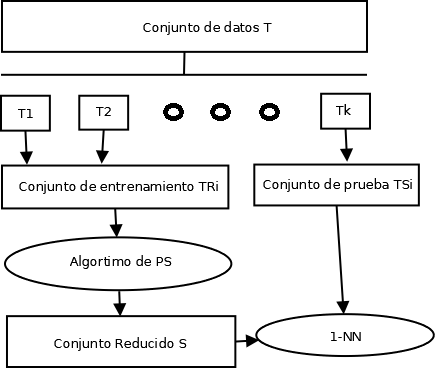
\includegraphics[scale=0.3]{classicCV.png}
%\caption[Validación cruzada]{Validación cruzada}
%\label{crossval}
%\end{figure}

\subsection{Estratificación}

La estratificación es una técnica propuesta por \emph{Cano, J. et al.} en \cite{cano2005stratification} para solventar el problema de aplicación de los algoritmos de PS a conjunto de datos muy grandes. Dicho problema viene dado porque la mayoría de los algoritmos de PS y metaheurísticas utilizadas son $O(n^2)$, donde $n$ es la cantidad de instancias del conjunto a procesar, y por lo tanto, tienen un problema de escalamiento cuando se utilizan con conjuntos de datos grandes.

Dado un conjunto de datos TR producto de la división hecha por un proceso de validación cruzada, la estratificación comienza con la división de TR en $k$ subconjuntos disjuntos, llamados estratos, $TR_1,TR_2,\dots,TR_k$ de aproximadamente el mismo tamaño. Luego, se aplica el algoritmo de PS directamente a cada uno de los $k$ subconjuntos seleccionados $TR_i$ para el entrenamiento, que más adelante forma subconjuntos reducidos $TRS_1,TRS_2,\dots,TRS_k$; acto seguido, se juntan todos los $TRS_i$ para formar el conjunto reducido S que va a ser usado por 1-NN para clasificar $TS$. La estratificación prueba ser un método efectivo, como lo demuestran en \cite{cano2005stratification}, ya que reduce la cantidad de instancias que debe tratar el algoritmo de PS a $TR/k$, por lo que la elección del número de estratos k se vuelve de especial importancia. En la figura \ref{strat-val} se muestra un esquema de cómo se aplica la estratificación, donde el estrato k es seleccionado como conjunto de prueba.

%\begin{figure}[h!]
%\centering
%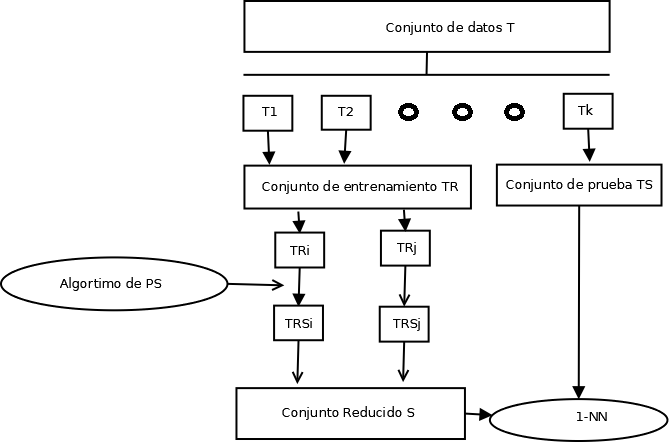
\includegraphics[scale=0.2]{stratCV.png}
%\caption[Estratificación]{Estratificación}
%\label{strat}
%\end{figure}


\begin{figure}[h!]

	\centering
	\subfigure[Validación cruzada]{\label{fig:a}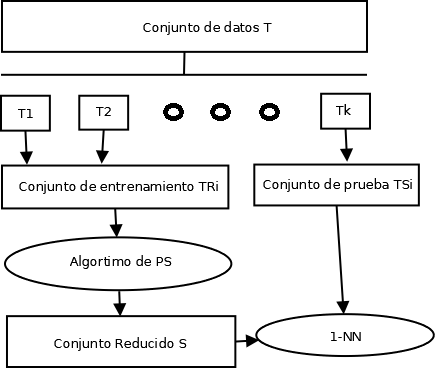
\includegraphics[scale=0.35]{classicCV.png}}
	\subfigure[Estratificación]{\label{fig:b}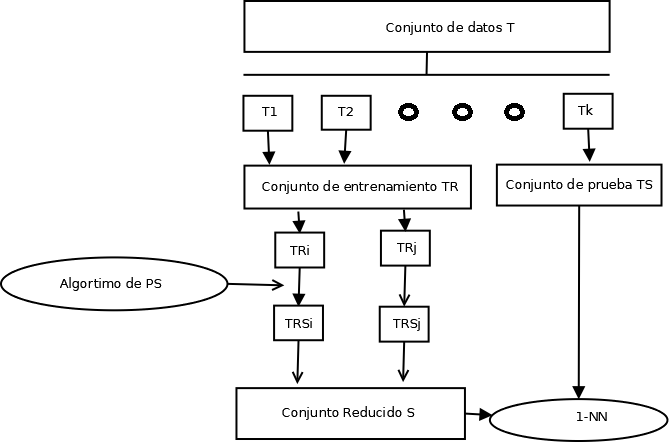
\includegraphics[scale=0.25]{stratCV.png}}

\caption{Validación cruzada y estratificación}
\label{strat-val}
\end{figure}

